% Author: Peter Steinbach
\documentclass[tikz]{standalone}
%\documentclass[dvisvgm]{standalone}
%\def\pgfsysdriver{pgfsys-tex4ht.def}
\usepackage{tikz}
\usepackage{units}
\usetikzlibrary{calc,trees,positioning,arrows.meta,chains,shapes.geometric,shapes.arrows,%
    decorations.pathreplacing,decorations.pathmorphing,shapes,%
    matrix,shapes.symbols,fit,backgrounds}

 \pgfdeclarelayer{back}
 \pgfsetlayers{background,back,main}


\makeatletter
\makeatother

\begin{document}


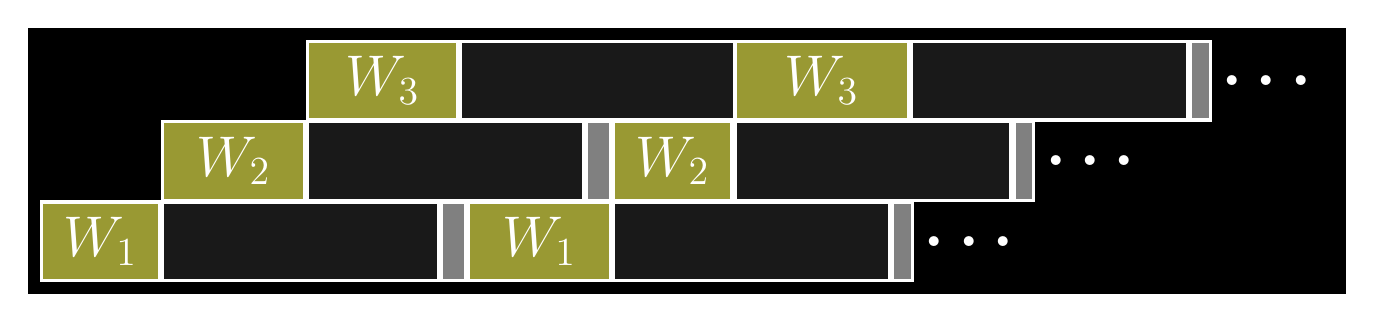
\begin{tikzpicture}[
  show background rectangle, 
  background rectangle/.style={fill=black},
  color=white,
  help lines/.style={color=lightgray,line width=.2pt},
  warp_work/.style={rectangle,very thick,inner sep=0pt,minimum height=1cm,fill=brown!80!green,draw=white,font=\huge,anchor=west},
  warp_delay/.style={rectangle,very thick,inner sep=0pt,minimum height=1cm,fill=gray!20!black,draw=white,font=\huge,anchor=west},
  warp_wait/.style={rectangle,very thick,inner sep=0pt,minimum height=1cm,fill=gray,draw=white,font=\huge,anchor=west}
  ]

%warp 1 
  \node (W_1_a) [warp_work,minimum width=1.5cm] at(0,.5) {$W_{1}$};
  \node (W_1_delay_a) [warp_delay,minimum width=3.5cm] at(W_1_a.east) {};
  \node (W_1_wait_a) [warp_wait,minimum width=.3cm] at(W_1_delay_a.east) {};

  \node (W_1_b) [warp_work,minimum width=1.8cm] at(W_1_wait_a.east) {$W_{1}$};
  \node (W_1_delay_b) [warp_delay,minimum width=3.5cm] at(W_1_b.east) {};
  \node (W_1_wait_b) [warp_wait,minimum width=.25cm] at(W_1_delay_b.east) {};

%warp 2 
  \node (W_2_a) [warp_work,minimum width=1.8cm] at($(W_1_a.north east)+(0,.5)$) {$W_{2}$};
  \node (W_2_delay_a) [warp_delay,minimum width=3.5cm] at(W_2_a.east) {};
  \node (W_2_wait_a) [warp_wait,minimum width=.3cm] at(W_2_delay_a.east) {};

  \node (W_2_b) [warp_work,minimum width=1.5cm] at(W_2_wait_a.east) {$W_{2}$};
  \node (W_2_delay_b) [warp_delay,minimum width=3.5cm] at(W_2_b.east) {};
  \node (W_2_wait_b) [warp_wait,minimum width=.25cm] at(W_2_delay_b.east) {};

%warp 3
  \node (W_3_a) [warp_work,minimum width=1.9cm] at($(W_2_a.north east)+(0,.5)$) {$W_{3}$};
  \node (W_3_delay_a) [warp_delay,minimum width=3.5cm] at(W_3_a.east) {};

  \node (W_3_b) [warp_work,minimum width=2.2cm] at($(W_2_b.north east)+(0,.5)$) {$W_{3}$};
  \node (W_3_delay_b) [warp_delay,minimum width=3.5cm] at(W_3_b.east) {};
  \node (W_3_wait_b) [warp_wait,minimum width=.25cm] at(W_3_delay_b.east) {};

  \node (W_3_dots) [font=\Huge,anchor=west] at(W_3_wait_b.east) {\bfseries{}\dots};
  \node (W_2_dots) [font=\Huge,anchor=west] at(W_2_wait_b.east) {\bfseries{}\dots};
  \node (W_1_dots) [font=\Huge,anchor=west] at(W_1_wait_b.east) {\bfseries{}\dots};

\end{tikzpicture}
\end{document}
